\section{Error Class Reference}
\label{classError}\index{Error@{Error}}
Stream-like class to print an error message to the app's console window Example:.  


{\tt \#include $<$Log.h$>$}

Inheritance diagram for Error:\nopagebreak
\begin{figure}[H]
\begin{center}
\leavevmode
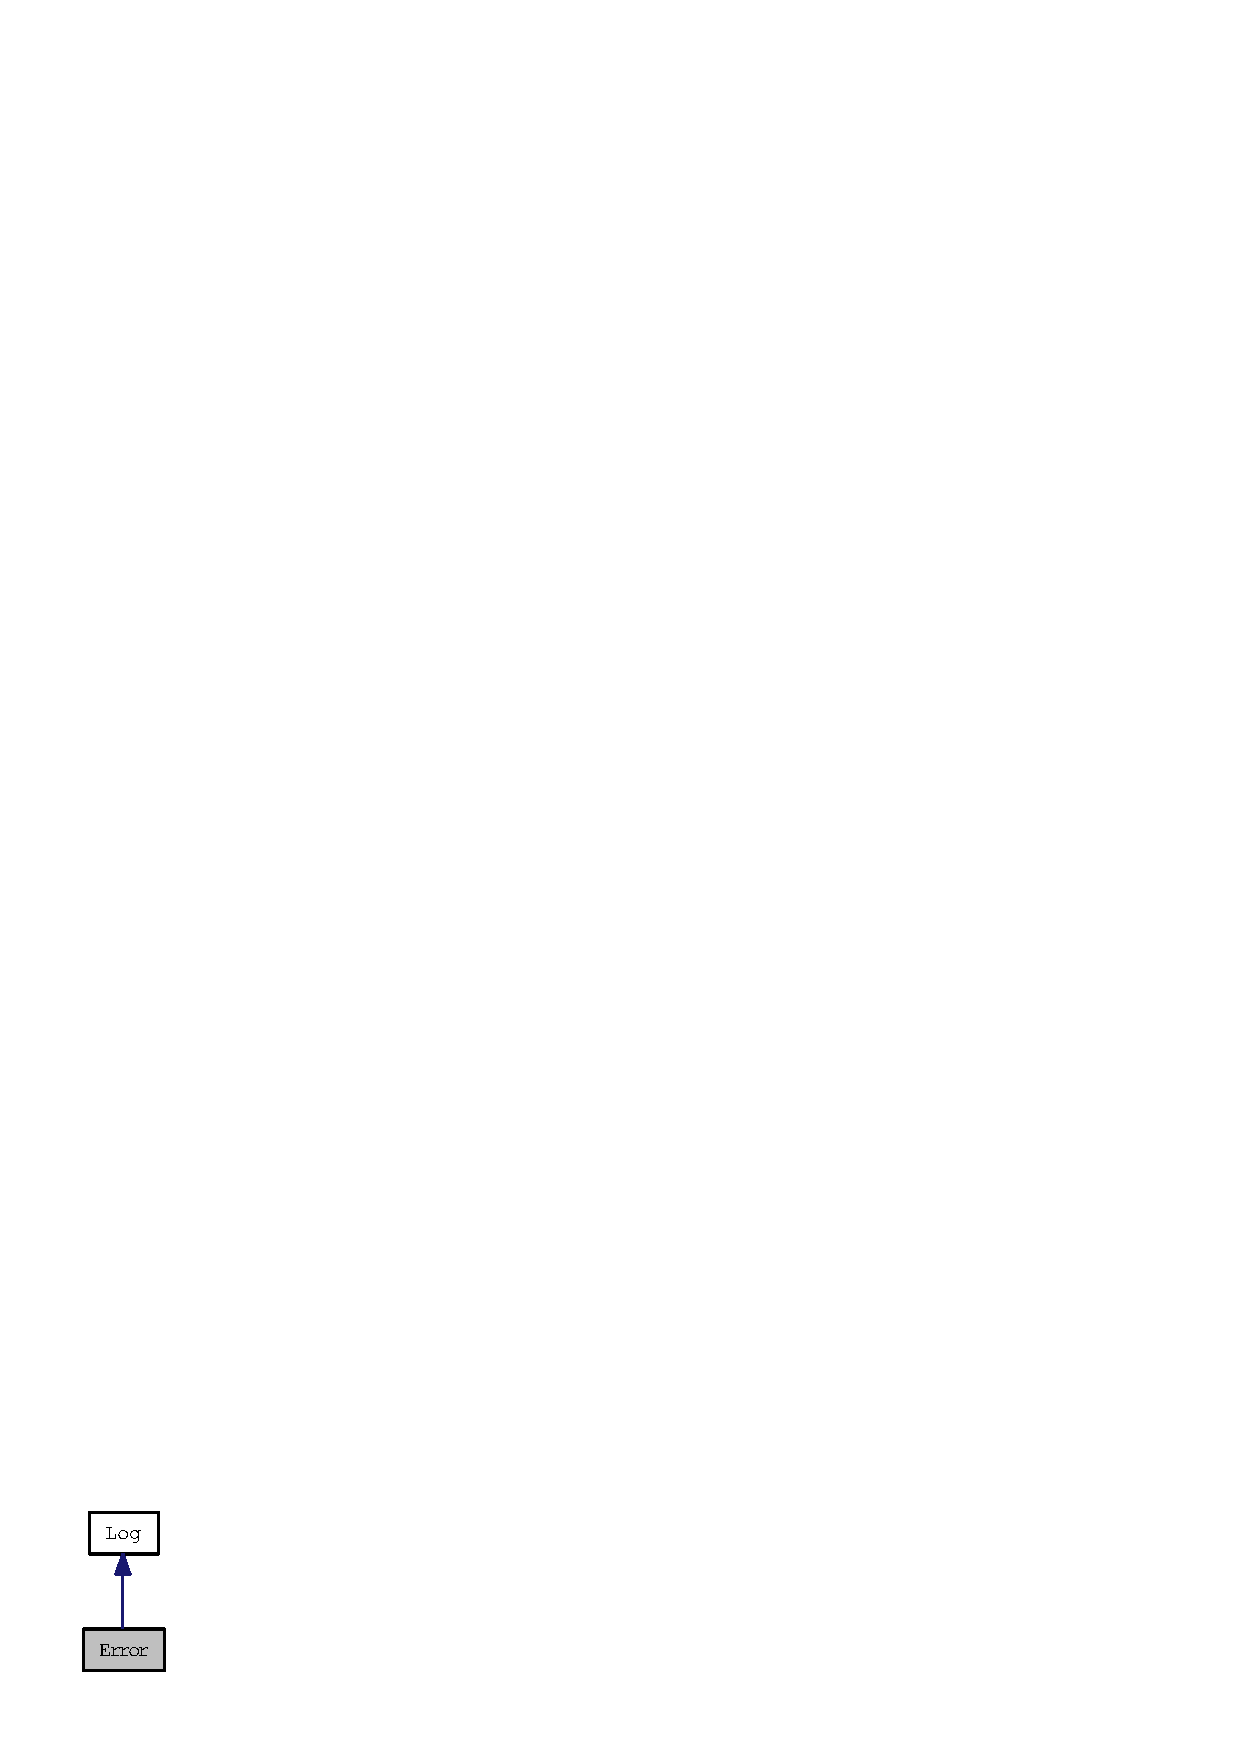
\includegraphics[width=41pt]{classError__inherit__graph}
\end{center}
\end{figure}
Collaboration diagram for Error:\nopagebreak
\begin{figure}[H]
\begin{center}
\leavevmode
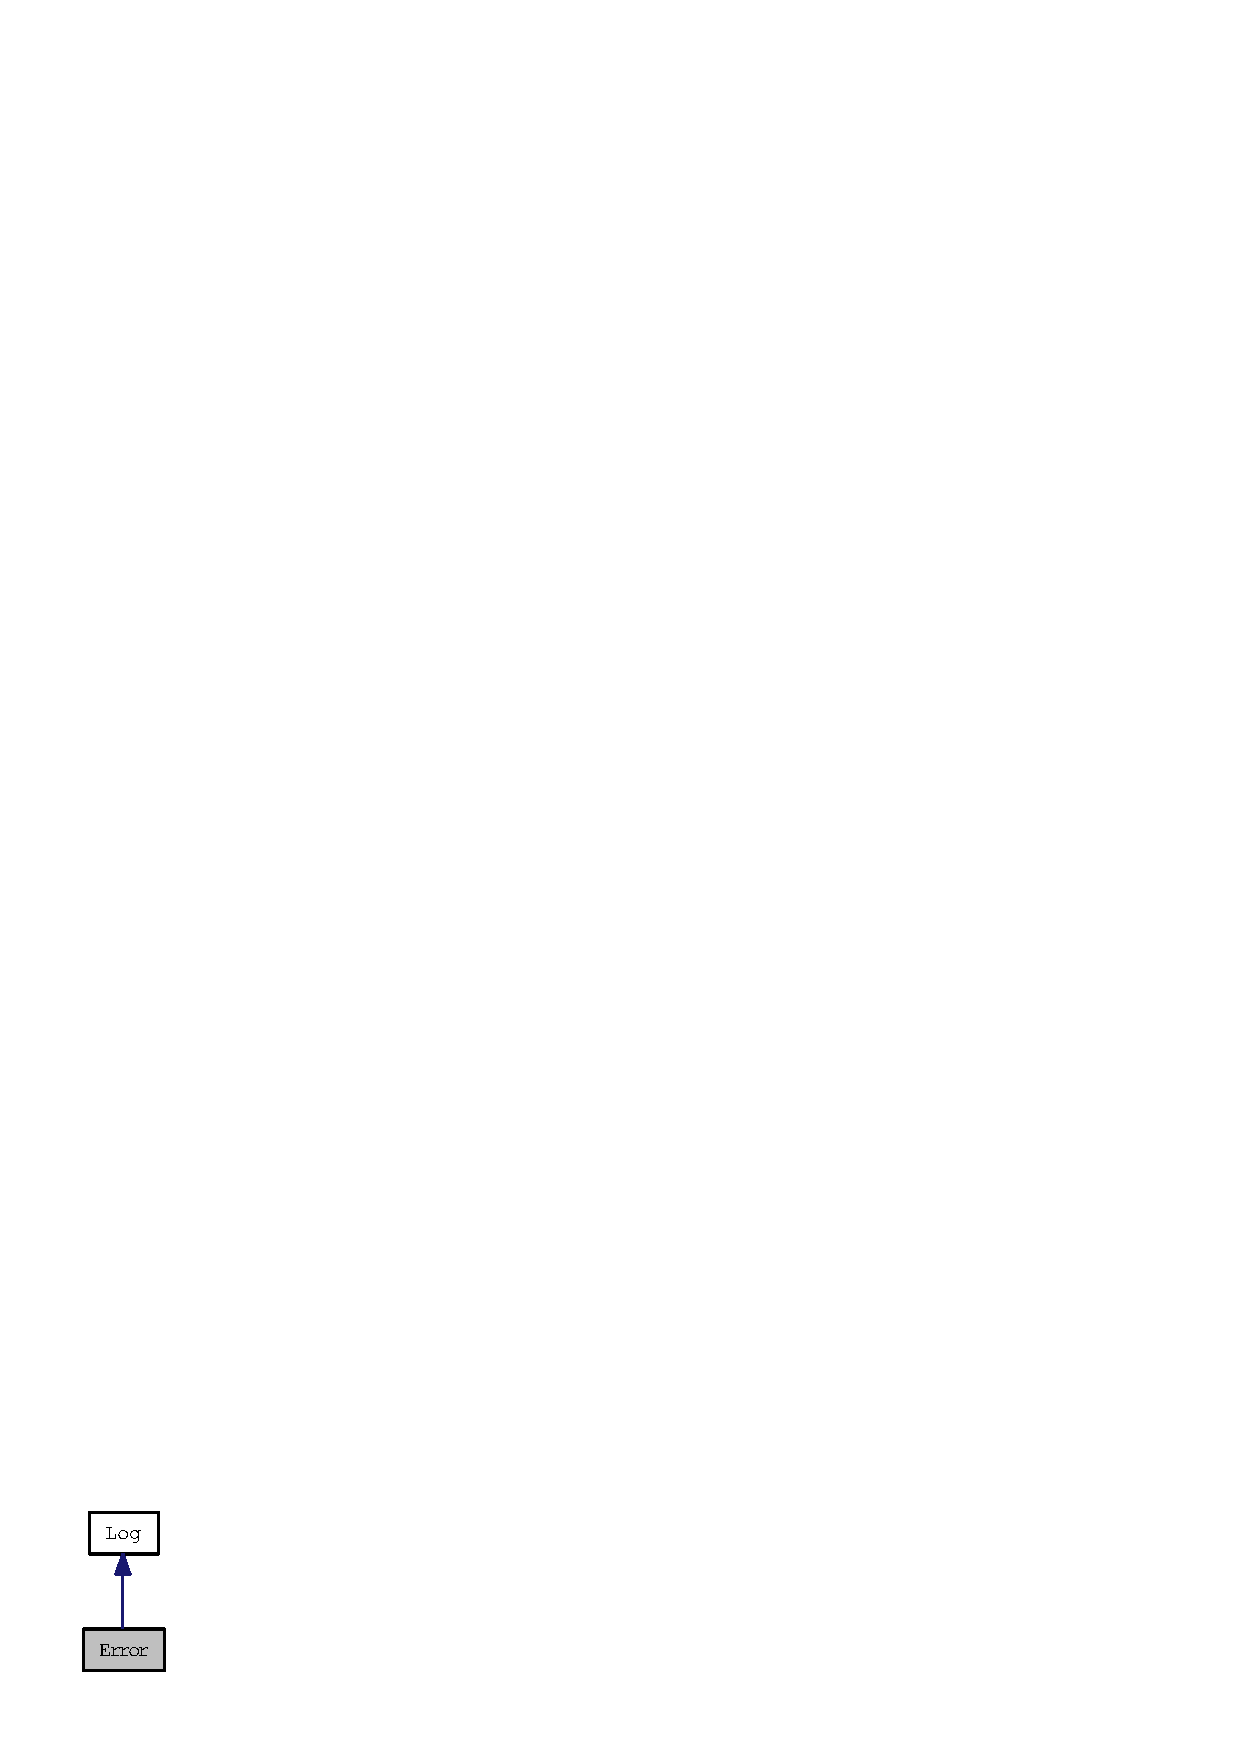
\includegraphics[width=41pt]{classError__coll__graph}
\end{center}
\end{figure}


\subsection{Detailed Description}
Stream-like class to print an error message to the app's console window Example:. 



\begin{Code}\begin{verbatim}        Error() << "This is an ERROR message!!"; // would print an error message to the console window
\end{verbatim}
\end{Code}

 

Definition at line 46 of file Log.h.

The documentation for this class was generated from the following files:\begin{CompactItemize}
\item 
Log.h\item 
Log.cpp\end{CompactItemize}
